% -- Document configuration
\documentclass{article}

% -- Input and language settings
% \usepackage[utf8]{inputenc}
\usepackage[spanish]{babel}
\decimalpoint                             % From babel package to use points instead of commas in decimals

% -- Page and line settings
\usepackage{geometry}
\geometry{letterpaper, 
    % margin=2cm, 
    left=3cm, right=3cm,
    top=1.2cm, bottom=1.2cm,
    includefoot, 
    includehead}
\renewcommand{\baselinestretch}{1.2}

% -- Required packages
\usepackage{xcolor}
\usepackage[many]{tcolorbox}
\usepackage{mathtools,amsfonts,amsmath}     % Loads amsmath if not already loaded
\allowdisplaybreaks                         % To allow page breaks if equations are too long
\usepackage[parfill]{parskip}               % No indent and separation lines for paragraphs
\usepackage{cancel}                         % To cancel math terms
\usepackage[shortlabels]{enumitem}          % To handle enumerations
\usepackage{tikz}
\usetikzlibrary{automata, arrows.meta, positioning}
\usepackage[mode=buildnew]{standalone}      % To import figures in standalone files
\usepackage[hidelinks]{hyperref}
\usepackage[spanish]{cleveref}              % To use autocompleted reference labels, language must be change as in babel package
\usepackage{caption}                        % Caption and subcaption to allow subfigures
\usepackage{subcaption}
\usepackage{float}                          % To specify the location of figures
\usepackage{multicol}                       % To use multicolumns
\usepackage[bottom]{footmisc}               % To locate footnotes at the bottom

% -- Title and heading settings
\usepackage{titling}
\usepackage{fancyhdr}
\pagestyle{fancy}

% -- Code and code formatting
\usepackage{minted}                         % To insert code
\usemintedstyle[julia]{gruvbox-light}       % Code theme and language
\definecolor{bg}{rgb}{0.98, 0.97, 0.88}     % Code block background

\usepackage{fontspec}                       % To allow the use of monospace fonts
\setmonofont{JuliaMono}[Path=./codefonts/, Extension=.ttf, UprightFont=*-Regular, ItalicFont=*-RegularItalic, Scale=0.75]

\usepackage{fancyvrb}                       % To change line number font
\renewcommand{\theFancyVerbLine}{\textcolor{gray}{\footnotesize\texttt{\arabic{FancyVerbLine}}}}

\definecolor{light-gray}{gray}{0.95}        % Color, box and style to show small code thingys inside normal text
\newcommand{\code}[1]{\colorbox{light-gray}{\texttt{#1}}}

% -- Bilbiography preferences
\usepackage[square,numbers]{natbib}
\bibliographystyle{unsrt}

% -- Footnotes without numbering
\newcommand\nnfootnote[1]{%
  \begin{NoHyper}
  \renewcommand\thefootnote{}\footnote{#1}%
  \addtocounter{footnote}{-1}%
  \end{NoHyper}
}

% -- Theorems
\newtheorem{theorem}{Theorem}

\lhead{\theinstitution\ -- \thedepartment}
\chead{}
\rhead{Programación para la IA\ -- \thetitle}
\lfoot{}
\cfoot{\thepage}
\rfoot{}

% -- Problem solution
\newenvironment{solution}
{\begin{quote}
\textbf{Solución:}\medskip

}
{

\hfill\rule{0.5\textwidth}{0.5pt}
\end{quote}}

% -- Equation result
\newcommand{\result}[1]
{
\tcbhighmath[colframe=white, colback=gray!15, sharp corners]
{#1}
}

% -- Function definitions
\newcommand{\dprod}[2]{{#1} \cdot {#2}}
\newcommand{\txtgray}[1]{\textcolor{gray}{#1}}

% -- Author information
\title{Actividad 5}
\author{Leonardo Flores Torres}
\newcommand\theinstitution{Universidad Veracruzana}
\newcommand\thedepartment{Inteligencia Artificial}
\newcommand\thecourse{Programación para la Inteligencia Artificial}

% -- Paths
% \newcommand\codelists{../programs/lists.rkt}

% Remove red color boxes of "syntax errors" in minted
\AtBeginEnvironment{minted}{%
  \renewcommand{\fcolorbox}[4][]{#4}}

% -- Document
\begin{document}

\thispagestyle{empty}

%Title
\begin{center}
\textsc{\theinstitution}\\[2mm]

\thedepartment

\rule{0.6\textwidth}{0.5pt}\\[2mm]

\thecourse \\[4mm]

{\Large \textbf{\thetitle}}\\[2mm]

\theauthor \\[2mm]

{\small \today}
\end{center}
\medskip

% -- 
\vspace{1cm}

Adaptar el algoritmo de Dijkstra para que trabaje en una rejilla donde se defina el punto inicial $(r_i, c_i)$ y el punto final $(r_f, c_f)$ y encuentre la ruta óptima con las siguientes variantes,
\begin{enumerate}
    \item usar 4 vecinos con distancias unitarias,
    \item usar 8 vecinos,
    \item incluir la posibilidad de encontrar obstáculos.
    \begin{solution}
        El módulo desarrollado, \code{ShortestPath}, para resolver esta actividad se muestra en el apéndice de este trabajo, en él se pueden observar mejor las restricciones para detectar vecinos de los pixeles aunque se agregará una breve explicación de esto en pseudocódigo. El algoritmo de Dijkstra no fue implementado sino que se utilizó una librería \cite{Graphs2021} ya desarrollada en \code{julia} que permite el uso de grafos y además incluye la implementación de distintos algoritmos de recorrido y búsqueda de los caminos más cortos, como lo es el de Dijkstra.

        Antes de comenzar a utilizar el módulo es importante pensar primero en cómo crear las relaciones que existen entre pixeles, en otras palabras, hay que idear de alguna manera como identificar los vecinos que un pixel tiene. El caso ideal es cuando el pixel del que se quiere encontrar los vecinos se encuentra en una posición como la que se muestra en la \cref{fig:ideal_pixel}.
        \begin{figure}[ht!]
            \centering
            \begin{subfigure}{0.4\textwidth}
                \centering
                \begin{tikzpicture}
                    % Neighbouring nodes
                    \fill[green!25] (1,0) rectangle (2,1);
                    \fill[green!25] (2,1) rectangle (3,2);
                    \fill[green!25] (1,2) rectangle (2,3);
                    \fill[green!25] (1,0) rectangle (2,1);
                    \fill[green!25] (0,1) rectangle (1,2);
                    % Grid
                    \draw[help lines, color=gray!35, dashed, step=1] (0,0) grid (4,4);
                    % Main node
                    \draw[fill=gray!75, draw=gray!85] (1,1) rectangle (2,2);
                    % Nodes ids
                    \node at (0.5,3.5) {1};
                    \node at (1.5,3.5) {2};
                    \node at (2.5,3.5) {3};
                    \node at (3.5,3.5) {4};
                    \node at (0.5,2.5) {5};
                    \node at (1.5,2.5) {6};
                    \node at (2.5,2.5) {7};
                    \node at (3.5,2.5) {8};
                    \node at (0.5,1.5) {9};
                    \node at (1.5,1.5) {10};
                    \node at (2.5,1.5) {11};
                    \node at (3.5,1.5) {12};
                    \node at (0.5,0.5) {13};
                    \node at (1.5,0.5) {14};
                    \node at (2.5,0.5) {15};
                    \node at (3.5,0.5) {16};
                \end{tikzpicture}
                \caption{Configuración de 4 vecinos.}
            \end{subfigure}
            \begin{subfigure}{0.4\textwidth}
                \centering
                \begin{tikzpicture}
                    % Neighbouring nodes
                    \fill[green!25] (0,0) rectangle (3,3);
                    % Grid
                    \draw[help lines, color=gray!35, dashed, step=1] (0,0) grid (4,4);
                    % Main node
                    \draw[fill=gray!75, draw=gray!85] (1,1) rectangle (2,2);
                    % Nodes ids
                    \node at (0.5,3.5) {1};
                    \node at (1.5,3.5) {2};
                    \node at (2.5,3.5) {3};
                    \node at (3.5,3.5) {4};
                    \node at (0.5,2.5) {5};
                    \node at (1.5,2.5) {6};
                    \node at (2.5,2.5) {7};
                    \node at (3.5,2.5) {8};
                    \node at (0.5,1.5) {9};
                    \node at (1.5,1.5) {10};
                    \node at (2.5,1.5) {11};
                    \node at (3.5,1.5) {12};
                    \node at (0.5,0.5) {13};
                    \node at (1.5,0.5) {14};
                    \node at (2.5,0.5) {15};
                    \node at (3.5,0.5) {16};
                \end{tikzpicture}
                \caption{Configuración de 8 vecinos.}
            \end{subfigure}
            \caption{Se muestra un cuadro en gris obscuro equivalente a un pixel y sus vecinos en gris claro en un arreglo representando a una imágen para ambas configuraciones de vecinos permitidas.}
            \label{fig:ideal_pixel}
        \end{figure}

        Se puede observar que no se está accediendo a los pixeles como si la imagen fuese un arreglo bidimensional, en realidad se hizo una transformación de los índices $(\text{row}, \text{col})$ de los pixeles de la imágen para relacionarlos con un identificador, $\text{id}$. Esta transformación es hecha a partir de 
        \begin{equation*}
            \text{id}(\text{row}, \text{col}) = \text{col} + n_c (\text{row} - 1),
        \end{equation*}
        donde $n_c$ es el número de columnas. Si por algún motivo fuese necesario regresar a la representación de $(\text{row}, \text{col})$, esto puede hacerse como
        \begin{equation*}
            \text{col} = 
            \begin{cases}
                n_c\ \hspace{1.5cm}\text{si id mod } n_c = 0 , \\
                \text{id mod } n_c \hspace{0.3cm}\text{ en cualquier otro caso.}
            \end{cases}
        \end{equation*}
        donde el primer caso es aquel cuando el $\text{id}$ corresponde a pixeles ubicados en la útila columna, y el segundo caso es cuando el $\text{id}$ corresponde a pixeles en cualquier otra columna diferente a la última. Por otro lado, calcular la fila es trivial si ya se conoce el identificador y la columna, solamente se despeja $\text{row}$ de la expresión para $\text{id}(\text{row}, \text{col})$.

        Independientemente de la configuración elegida, ya sea la de 4 u 8 vecinos, es importante reconocer todos los escenarios cuando el pixel se encuentra en una posición en la que no tiene acceso a todos los pixeles que tendría en el caso ideal, esto sucede cuando dicho pixel se encuentra en los bordes de la imágen. El primer escenario considerado sucede cuando se quieren encontrar los vecinos de un pixel a su derecha o a su izquierda, como en la \cref{fig:vecinos_horizontal}. Para este caso hay dos restricciones evidentes, cuando el pixel se encuentra en la primera columna, y cuando lo está en la última columna.
        \begin{figure}[ht!]
            \centering
            \begin{tikzpicture}
                % Danger zones
                \fill[red!15] (3,0) rectangle (4,4);
                \fill[red!15] (0,0) rectangle (1,4);
                % Bottom left neighbors
                \fill[green!25] (1,0) rectangle (2,1);
                \fill[red!35] (-1,0) rectangle (0,1);
                % Top right neighbors
                \fill[green!25] (2,2) rectangle (3,3);
                \fill[red!35] (4,2) rectangle (5,3);
                % Grid
                \draw[help lines, color=gray!35, dashed, step=1] (0,0) grid (4,4);
                % Main pixels
                \draw[fill=gray!75, draw=gray!85] (3,2) rectangle (4,3);
                \draw[fill=gray!75, draw=gray!85] (0,0) rectangle (1,1);
                % Nodes ids
                \node at (0.5,3.5) {1};
                \node at (1.5,3.5) {2};
                \node at (2.5,3.5) {3};
                \node at (3.5,3.5) {4};
                \node at (0.5,2.5) {5};
                \node at (1.5,2.5) {6};
                \node at (2.5,2.5) {7};
                \node at (3.5,2.5) {8};
                \node at (0.5,1.5) {9};
                \node at (1.5,1.5) {10};
                \node at (2.5,1.5) {11};
                \node at (3.5,1.5) {12};
                \node at (0.5,0.5) {13};
                \node at (1.5,0.5) {14};
                \node at (2.5,0.5) {15};
                \node at (3.5,0.5) {16};
            \end{tikzpicture}
            \caption{Vecinos no permitidos, en dirección horizontal, de un pixel dado.}
            \label{fig:vecinos_horizontal}
        \end{figure}

        De esta manera podemos decir que si el módulo del identificador de un pixel respecto al número total de columnas $n_c$ es igual a cero no tiene vecino a la derecha, o si el módulo del identificador menos 1 respecto $n_c$ es cero entonces no tiene vecino a la izquierda. Esto se puede ver expresado en el pseudocódigo mostrado a continuación (para todos los snippets de pseudocódigo \code{nc} es el número de columnas y \code{nr} el de filas):
        \begin{minted}[
            frame=none,
            autogobble,
            obeytabs=false,
            breaklines,
            tabsize=4,
            linenos=true,
            % numbersep=-10pt,
            baselinestretch=1,
            firstnumber=1,
            bgcolor=bg!70,
            ]{julia}
            # Pseudocodigo
            # Vecino a la derecha
            if id % nc != 0
                agrega (id + 1) como vecino
            end if
            # Vecino a la izquierda
            if (id - 1) % nc != 0
                agrega (id - 1) como vecino
            end if
        \end{minted}

        El siguiente escenario se muestra en la \cref{fig:vecinos_vertical} donde la búsqueda de vecinos para un pixel dado se realiza verticalmente, esto es, se buscan los vecinos que queden inmediatanente arriba y abajo de un cierto pixel. Para este caso se observa que hay dos restricciones, una de ellas es cuando el pixel se encuentra en la primera fila y la otra es cuando lo está en la última fila ya que los pixeles en la primera fila no tienen vecinos arriba de ellos, mientras que los que están en la última fila no tienen vecinos abajo.
        \begin{figure}[ht!]
            \centering
            \begin{tikzpicture}
                % Danger zones
                \fill[red!15] (0,0) rectangle (4,1);
                \fill[red!15] (0,3) rectangle (4,4);
                % Bottom left neighbors
                \fill[green!25] (1,1) rectangle (2,2);
                \fill[red!35] (1,-1) rectangle (2,0);
                % Top right neighbors
                \fill[green!25] (2,2) rectangle (3,3);
                \fill[red!35] (2,4) rectangle (3,5);
                % Grid
                \draw[help lines, color=gray!35, dashed, step=1] (0,0) grid (4,4);
                % Main pixels
                \draw[fill=gray!75, draw=gray!85] (2,3) rectangle (3,4);
                \draw[fill=gray!75, draw=gray!85] (1,0) rectangle (2,1);
                % Nodes ids
                \node at (0.5,3.5) {1};
                \node at (1.5,3.5) {2};
                \node at (2.5,3.5) {3};
                \node at (3.5,3.5) {4};
                \node at (0.5,2.5) {5};
                \node at (1.5,2.5) {6};
                \node at (2.5,2.5) {7};
                \node at (3.5,2.5) {8};
                \node at (0.5,1.5) {9};
                \node at (1.5,1.5) {10};
                \node at (2.5,1.5) {11};
                \node at (3.5,1.5) {12};
                \node at (0.5,0.5) {13};
                \node at (1.5,0.5) {14};
                \node at (2.5,0.5) {15};
                \node at (3.5,0.5) {16};
            \end{tikzpicture}
            \caption{Vecinos no permitidos, en dirección vertical, de un pixel dado.}
            \label{fig:vecinos_vertical}
        \end{figure}

        Así, se puede decir que los pixeles con identificadores que tengan valor menor o igual al número total de columnas no tendrán vecinos sobre de ellos, mientras que aquellos pixeles con identificadores en la última fila no tendrán vecinos debajo de ellos. Lo interesante es ver que si un pixel tiene un vecino arriba, este vecino tendrá como identificador el identificador del pixel menos el número de columnas de la imágen, $\text{id}_{\text{pixel}} - n_c$. Algo similar sucede cuando se buscan vecinos abajo, el identificador del vecino es el del pixel agregandole el número de columnas, $\text{id}_{\text{pixel}} + n_c$ . Esto se puede representar de la siguiente manera en pseudocódigo:
        \begin{minted}[
            frame=none,
            autogobble,
            obeytabs=false,
            breaklines,
            tabsize=4,
            linenos=true,
            % numbersep=-10pt,
            baselinestretch=1,
            firstnumber=1,
            bgcolor=bg!70,
            ]{julia}
            # Pseudocodigo
            # Vecino arriba
            if id > nc
                agrega (id - nc) como vecino
            end if
            # Vecino abajo
            if id <= nc * (nr - 1)
                agrega (id + nc) como vecino
            end if
        \end{minted}

        Un penúltimo escenario es el mostrado en la \cref{fig:vecinos_diag_op1} donde se muestra la cuadrícula dos veces debido a que se puede dar el caso de caer en una de ellas. Por ejemplo, se puede dar el caso de que el pixel del que se quieren obtener sus vecinos se encuentre en la primera columna o en la última fila, en ambos casos no hay vecino de dicho pixel abajo a la izquierda. El otro caso es si el pixel se encuentra en la primera fila o en la última columna, donde no habría disponible un vecino arriba a la derecha.
        \begin{figure}[ht!]
            \centering
            \begin{subfigure}{0.4\textwidth}
                \centering
                \begin{tikzpicture}
                    % Danger zones
                    \fill[red!15] (0,0) rectangle (4,1);
                    \fill[red!15] (0,0) rectangle (1,4);
                    % Bottom left neighbors
                    \fill[green!25] (1,2) rectangle (2,3);
                    \fill[red!35] (-1,0) rectangle (0,1);
                    % Top right neighbors
                    \fill[green!25] (2,2) rectangle (3,3);
                    \fill[red!35] (4,4) rectangle (5,5);
                    % Grid
                    \draw[help lines, color=gray!35, dashed, step=1] (0,0) grid (4,4);
                    % Main pixels
                    \draw[fill=gray!75, draw=gray!85] (3,3) rectangle (4,4);
                    \draw[fill=gray!75, draw=gray!85] (0,1) rectangle (1,2);
                    % Nodes ids
                    \node at (0.5,3.5) {1};
                    \node at (1.5,3.5) {2};
                    \node at (2.5,3.5) {3};
                    \node at (3.5,3.5) {4};
                    \node at (0.5,2.5) {5};
                    \node at (1.5,2.5) {6};
                    \node at (2.5,2.5) {7};
                    \node at (3.5,2.5) {8};
                    \node at (0.5,1.5) {9};
                    \node at (1.5,1.5) {10};
                    \node at (2.5,1.5) {11};
                    \node at (3.5,1.5) {12};
                    \node at (0.5,0.5) {13};
                    \node at (1.5,0.5) {14};
                    \node at (2.5,0.5) {15};
                    \node at (3.5,0.5) {16};
                \end{tikzpicture}
            \end{subfigure}
            \begin{subfigure}{0.4\textwidth}
                \centering
                \begin{tikzpicture}
                    % Danger zones
                    \fill[red!15] (0,3) rectangle (4,4);
                    \fill[red!15] (3,0) rectangle (4,4);
                    % Bottom left neighbors
                    \fill[green!25] (1,2) rectangle (2,3);
                    \fill[red!35] (-1,0) rectangle (0,1);
                    % Top right neighbors
                    \fill[green!25] (2,2) rectangle (3,3);
                    \fill[red!35] (4,4) rectangle (5,5);
                    % Grid
                    \draw[help lines, color=gray!35, dashed, step=1] (0,0) grid (4,4);
                    % Main pixels
                    \draw[fill=gray!75, draw=gray!85] (3,3) rectangle (4,4);
                    \draw[fill=gray!75, draw=gray!85] (0,1) rectangle (1,2);
                    % Nodes ids
                    \node at (0.5,3.5) {1};
                    \node at (1.5,3.5) {2};
                    \node at (2.5,3.5) {3};
                    \node at (3.5,3.5) {4};
                    \node at (0.5,2.5) {5};
                    \node at (1.5,2.5) {6};
                    \node at (2.5,2.5) {7};
                    \node at (3.5,2.5) {8};
                    \node at (0.5,1.5) {9};
                    \node at (1.5,1.5) {10};
                    \node at (2.5,1.5) {11};
                    \node at (3.5,1.5) {12};
                    \node at (0.5,0.5) {13};
                    \node at (1.5,0.5) {14};
                    \node at (2.5,0.5) {15};
                    \node at (3.5,0.5) {16};
                \end{tikzpicture}
            \end{subfigure}
            \caption{Vecinos no permitidos, en una posible dirección vertical, de un pixel dado.}
            \label{fig:vecinos_diag_op1}
        \end{figure}

        Las restricciones que surgen a causa de esto son combinaciones de las ya definidas anteriormente. Todos los pixeles en la zona roja de la primera columna y la última fila no pueden tener vecinos abajo a la izquierda, y todos los pixeles en la zona roja de la primera fila y última columna no pueden tener vecinos arriba a la derecha, así que se combinan las restricciones pertinentes. Esto se puede escribir en pseudocódigo como se muestra a continuación:
        \begin{minted}[
            frame=none,
            autogobble,
            obeytabs=false,
            breaklines,
            tabsize=4,
            linenos=true,
            % numbersep=-10pt,
            baselinestretch=1,
            firstnumber=1,
            bgcolor=bg!70,
            ]{julia}
            # Pseudocodigo
            # Vecino arriba a la derecha
            if id % nc !=0 && id > nc
                agrega (id - nc + 1) como vecino
            end if
            # Vecino abajo a la izquierda
            if (id - 1) % nc != 0 && id <= nc * (nr - 1)
                agrega (id + nc - 1) como vecino
            end if
        \end{minted}

        El último escenario es aquel en que el pixel del que se quieren saber sus vecinos se encuentra en la primera columna o en la primera fila, y también se puede dar que dicho pixel se encuentre en la última fila o última columna. Para ambos casos se hace una combinación de las reglas más simples ya definidas.
        \begin{figure}[ht!]
            \centering
            \begin{subfigure}{0.4\textwidth}
                \centering
                \begin{tikzpicture}
                    % Danger zones
                    \fill[red!15] (0,3) rectangle (4,4);
                    \fill[red!15] (0,0) rectangle (1,4);
                    % Left neighbors
                    \fill[green!25] (1,1) rectangle (2,2);
                    \fill[red!35] (-1,3) rectangle (0,4);
                    % Right neighbors
                    \fill[green!25] (2,2) rectangle (3,3);
                    \fill[red!35] (4,0) rectangle (5,1);
                    % Grid
                    \draw[help lines, color=gray!35, dashed, step=1] (0,0) grid (4,4);
                    % Main pixels
                    \draw[fill=gray!75, draw=gray!85] (3,1) rectangle (4,2);
                    \draw[fill=gray!75, draw=gray!85] (0,2) rectangle (1,3);
                    % Nodes ids
                    \node at (0.5,3.5) {1};
                    \node at (1.5,3.5) {2};
                    \node at (2.5,3.5) {3};
                    \node at (3.5,3.5) {4};
                    \node at (0.5,2.5) {5};
                    \node at (1.5,2.5) {6};
                    \node at (2.5,2.5) {7};
                    \node at (3.5,2.5) {8};
                    \node at (0.5,1.5) {9};
                    \node at (1.5,1.5) {10};
                    \node at (2.5,1.5) {11};
                    \node at (3.5,1.5) {12};
                    \node at (0.5,0.5) {13};
                    \node at (1.5,0.5) {14};
                    \node at (2.5,0.5) {15};
                    \node at (3.5,0.5) {16};
                \end{tikzpicture}
            \end{subfigure}
            \begin{subfigure}{0.4\textwidth}
                \centering
                \begin{tikzpicture}
                    % Danger zones
                    \fill[red!15] (0,0) rectangle (4,1);
                    \fill[red!15] (3,0) rectangle (4,4);
                    % Left neighbors
                    \fill[green!25] (1,1) rectangle (2,2);
                    \fill[red!35] (-1,3) rectangle (0,4);
                    % Right neighbors
                    \fill[green!25] (2,2) rectangle (3,3);
                    \fill[red!35] (4,0) rectangle (5,1);
                    % Grid
                    \draw[help lines, color=gray!35, dashed, step=1] (0,0) grid (4,4);
                    % Main pixels
                    \draw[fill=gray!75, draw=gray!85] (3,1) rectangle (4,2);
                    \draw[fill=gray!75, draw=gray!85] (0,2) rectangle (1,3);
                    % Nodes ids
                    \node at (0.5,3.5) {1};
                    \node at (1.5,3.5) {2};
                    \node at (2.5,3.5) {3};
                    \node at (3.5,3.5) {4};
                    \node at (0.5,2.5) {5};
                    \node at (1.5,2.5) {6};
                    \node at (2.5,2.5) {7};
                    \node at (3.5,2.5) {8};
                    \node at (0.5,1.5) {9};
                    \node at (1.5,1.5) {10};
                    \node at (2.5,1.5) {11};
                    \node at (3.5,1.5) {12};
                    \node at (0.5,0.5) {13};
                    \node at (1.5,0.5) {14};
                    \node at (2.5,0.5) {15};
                    \node at (3.5,0.5) {16};
                \end{tikzpicture}
            \end{subfigure}
            \caption{Vecinos no permitidos, en una segunda posible dirección vertical, de un pixel dado.}
            \label{fig:vecinos_diag_op2}
        \end{figure}
        
        El pseudocódigo es similar al anterior, y se muestra a continuación:
        \begin{minted}[
            frame=none,
            autogobble,
            obeytabs=false,
            breaklines,
            tabsize=4,
            linenos=true,
            % numbersep=-10pt,
            baselinestretch=1,
            firstnumber=1,
            bgcolor=bg!70,
            ]{julia}
            # Pseudocodigo
            # Vecino arriba a la izquierda
            if (id - 1) % nc != 0 && id > nc
                agrega (id - nc - 1) como vecino
            end if
            # Vecino abajo a la derecha
            if id % nc != 0 && id <= nc * (nr - 1)
                agrega (id + nc + 1) como vecino
            end if
        \end{minted}
        No se especifíca en el pseudocódigo cómo o en dónde agregar a los vecinos, lo importante de esto es saber reconocer cuales son las restricciones para hacerlo, y el lector decidirá la mejor manera de realizar su propia implementación con la estructura de datos que desee. La razón por la que se eligió cambiar la representación del problema fue debido a que si no se hacía se tendría que haber utilizado dos \code{for-loop}'s anidados para iterar sobre todas las columnas y todas las filas. Aunque no representa una carga computacional pesada hacer esto para este problema en especifíco, lo consideré pertinente tomando en cuenta que se trata del curso de \textit{Análisis de Algoritmos} y quisiera poner en práctica lo aprendido siempre que me sea posible.

        La manera de utilizar el módulo, \code{ShortestPath}, en el \code{REPL} de \code{julia} se muestra a continuación. Primero se define el tamaño de la rejilla en \code{nrows} y \code{ncols}, y con estas variables se computa la representación de índices de los elementos de la rejilla, aunque resulta ser impractica de visualizar mientras más el número más vecinos hay en total dentro de la vecindad.
        \begin{minted}[
            frame=none,
            autogobble,
            obeytabs=false,
            breaklines,
            tabsize=4,
            linenos=true,
            % numbersep=-10pt,
            baselinestretch=1,
            firstnumber=1,
            bgcolor=bg!70,
            ]{julia}
            julia> using ShortestPath; sp = ShortestPath;
            julia> nrows = 40; ncols = 40;
            julia> idarray = [i for i in 1:(ncols * nrows)] |> x -> reshape(x, ncols, nrows) |> transpose;
            julia> start = [10, 3]; finish = [35, 37];
        \end{minted}

        Una vecindad es el nombre dado a la rejilla tomando en cuenta los puntos libres por los que se puede transitar, y los obstáculos, que son puntos imposibles de alcanzar. Además, los obstáculos se eligen de pixeles de manera aleatoria de la rejilla inicialmente libre, esto quiere decir que todos los pixeles son alzancables al inicio, se hace un muestreo aleatorio y aquellos elegidos cambian su estado a obstáculos. El argumento \code{obsdensity} de la función \code{neighborhood} indica la densidad de obstáculos deseada entre $[0, 1]$. 

        Se computó una vecindad con los puntos de partida inicial y final mostrados en \code{start} y \code{finish}, respectivamente, y una densidad de obstáculos del $0.25$. También se hizo una copia profunda de la vecindad \code{nh} en \code{nhdiag} ya que se obtuvieron las matrices de adyacencia para los casos donde el movimiento se puede dar sin y con diagonales en la misma rejilla, para 4 y 8 vecinos, respectivamente.
        \begin{minted}[
            frame=none,
            autogobble,
            obeytabs=false,
            breaklines,
            tabsize=4,
            linenos=true,
            % numbersep=-10pt,
            baselinestretch=1,
            firstnumber=last,
            bgcolor=bg!70,
            ]{julia}
            julia> nh, obs = sp.neighborhood(nrows, ncols; start=start, finish=finish, obsdensity=0.25); sp.visualize(nh)
            julia> nhdiag = deepcopy(nh);
            julia> adjmat = sp.adjacencyMatrix(nrows, ncols; obstacles=obs, allowdiags=false);
            julia> adjmatdiag = sp.adjacencyMatrix(nrows, ncols; obstacles=obs, allowdiags=true);
        \end{minted}

        Las matrices de adyacencia guardadas en las variables \code{adjmat} y \code{adjmatdiag} requieren como argumentos la lista de obstáculos en \code{obstacles}, si las diagonales son permitidas o no en \code{allowdiags}, y el número de filas y de columnas. Estos dos primeros argumentos son posicionales mientras que los primeros dos mencionados son argumentos de palabra clave, se observa la división entre un tipo de argumentos y otro con un \code{;} dentro de los argumentos de una función.

        Posteriormente se obtienen los caminos y las distancias de esos caminos con la función \code{findPath}; se computaron los caminos sin diagonales en \code{path} y con diagonales en \code{pathdiag}, con sus repectivas matrices de adyacencia. Para terminar, los caminos se usan para cambiar el estado de los pixeles en las vecindades \code{nh} y \code{nhdiag} con la función \code{updateneighborhood!}. Nótese que la función lleva un signo de admiración \code{!} al final de su nombre para denotar que es una función que modifica alguno de sus argumentos.
        \begin{minted}[
            frame=none,
            autogobble,
            obeytabs=false,
            breaklines,
            tabsize=4,
            linenos=true,
            % numbersep=-10pt,
            baselinestretch=1,
            firstnumber=last,
            bgcolor=bg!70,
            ]{julia}
            julia> path, dist = sp.findPath(adjmat, ncols; start=start, finish=finish);
            julia> pathdiag, distdiag = sp.findPath(adjmatdiag, ncols; start=start, finish=finish);
            julia> sp.updateneighborhood!(nhdiag, pathdiag); sp.visualize(nhdiag)
            julia> sp.updateneighborhood!(nh, path); sp.visualize(nh)
            julia> dist
            59.0
            julia> distdiag
            46.11269837220809
        \end{minted}

        \begin{figure}[ht!]
            \centering
            \begin{subfigure}{0.4\textwidth}
                \centering
                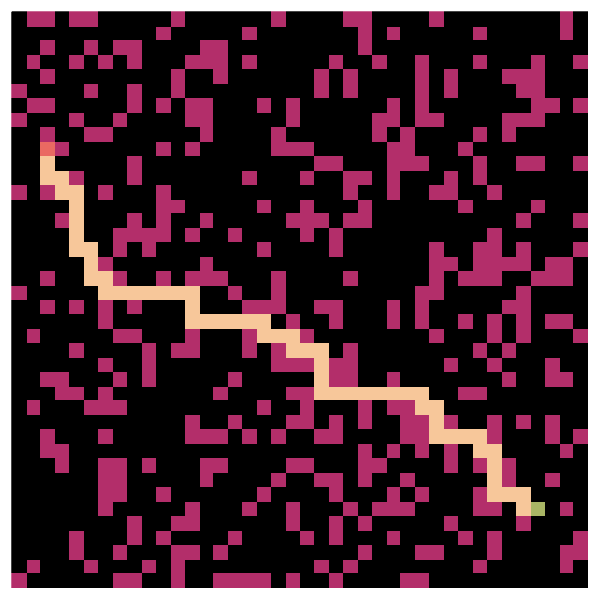
\includegraphics[scale=0.3]{../figures/path_01.png}
                \caption{4 vecinos (diagonales no permitidas); $\text{distancia} = 59 u$.}
                \label{fig:nodiags_obs_25percent_40x40}
            \end{subfigure}
            \hspace{1cm}
            %
            \begin{subfigure}{0.4\textwidth}
                \centering
                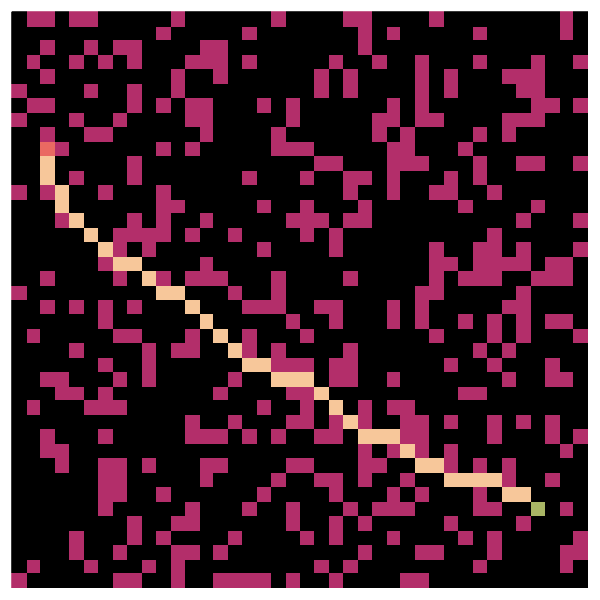
\includegraphics[scale=0.3]{../figures/path_01_diag.png}
                \caption{8 vecinos (diagonales permitidas); $\text{distancia} = 46.1126 u$.}
                \label{fig:diags_obs_25percent_40x40}
            \end{subfigure}
            \caption{Rejilla de $40 \times 40$ con una densidad de obstáculos al $25\%$.}
            \label{fig:rejilla_40x40}
        \end{figure}

        En la \cref{fig:rejilla_40x40} se muestran las imágenes para una rejilla de $40 \times 40$ incluyendo el caso en que el movimiento hacia vecinos solamente se da horizontal y verticalmente, \cref{fig:nodiags_obs_25percent_40x40}, y el caso en que el movimiento diagonal está permitido, \cref{fig:diags_obs_25percent_40x40}. Las distancias del recorrido en cada una de ellas son de $50$ unidades sin diagonales en la \cref{fig:nodiags_obs_25percent_40x40}, y de $46.11$ unidades considerando diagonales en la \cref{fig:diags_obs_25percent_40x40}.

        Los pixeles mostrados en color \tikz{\fill[black] (0,0) rectangle (0.3,0.3)} son los pixeles libres por los que se puede transitar mientras que los mostrados de color los pixeles de color \tikz{\fill[color_obstacle] (0,0) rectangle (0.3,0.3)} son los obstáculos; el pixel de color \tikz{\fill[color_start] (0,0) rectangle (0.3,0.3)} es el punto de partida definido en \code{start}, el pixel de color \tikz{\fill[color_finish] (0,0) rectangle (0.3,0.3)} es el punto de llegada definido en \code{finish}, y los pixeles de color \tikz{\fill[color_path] (0,0) rectangle (0.3,0.3)} muestran el camino atravesado para llegar a la meta.

        Esta implementación permite utilizar dimensiones para la rejilla diferentes de $n \times n$, esto quiere decir que se pueden elegir un número diferente de filas que de columnas, y viceversa. Un ejemplo de esto se muestra en la \cref{fig:rejilla_20x35}, con 20 filas y 35 columnas. El camino sin diagonales permitidas es de 50 unidades, mientras que aquel en que se permiten las diagonales tiene longitud de 36.87 unidades.
        \begin{figure}[ht!]
            \centering
            \begin{subfigure}{0.4\textwidth}
                \centering
                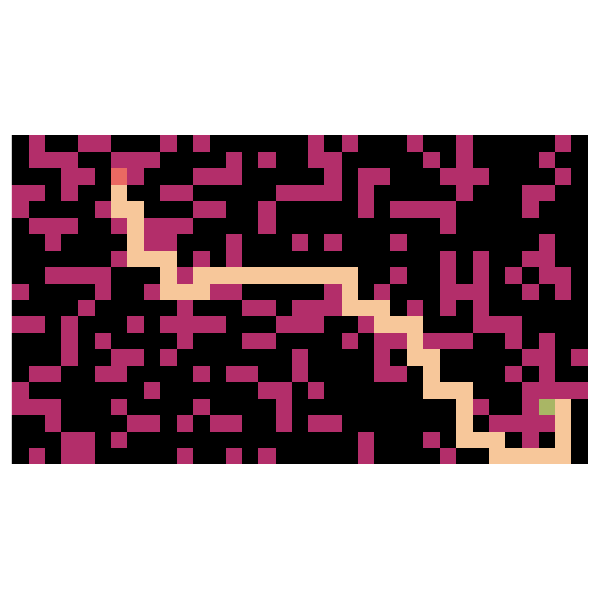
\includegraphics[scale=0.3]{../figures/path_02.png}
                \caption{4 vecinos (diagonales no permitidas); $\text{distancia} = 50 u$.}
            \end{subfigure}
            \hspace{1cm}
            %
            \begin{subfigure}{0.4\textwidth}
                \centering
                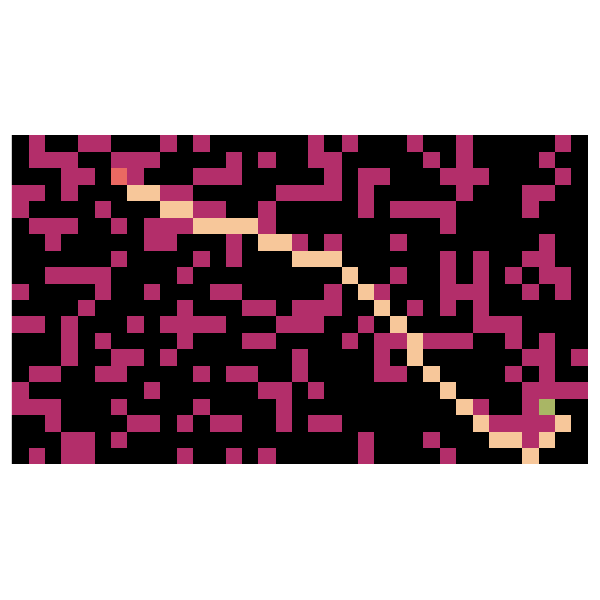
\includegraphics[scale=0.3]{../figures/path_02_diag.png}
                \caption{8 vecinos (diagonales no permitidas); $\text{distancia} = 36.87 u$.}
            \end{subfigure}
            \caption{Rejilla de $20 \times 35$ con una densidad de obstáculos del $30\%$.}
            \label{fig:rejilla_20x35}
        \end{figure}

        Quisiera agregar un par de comentarios extras acerca de la matriz de adyacencia, hablar acerca de porqué la representación elegida es útil. Lo primero es que la matriz de adyacencia es una matriz cuadrada de $n \times n$ donde $n$ es el número de pixeles dentro de la imágen independientemente de si son o no obstáculos. La representación elegida a partir de identificadores permite fácilmente acceder a un arreglo bidimensional tomando los identificadores como índices de una matriz, la matriz de adyacencia. Por ejemplo,
        \begin{equation*}
        \begin{blockarray}{c c c c c c c}
            & 1 & 2 & 3 & 4 & \hdots & n \\
            \begin{block}{c (c c c c c c)}
                1 & v(1,1) & v(1,2) & v(1,3) & v(1,4) & \hdots & v(1,n) \\
                2 & v(2,1) & v(2,2) & v(2,3) & v(2,4) & \hdots & v(2,n) \\
                3 & v(3,1) & v(3,2) & v(3,3) & v(3,4) & \hdots & v(3,n) \\
                4 & v(4,1) & v(4,2) & v(4,3) & v(4,4) & \hdots & v(4,n) \\
                \vdots & \vdots & \vdots & \vdots & \vdots & \ddots & \vdots \\
                n & v(n,1) & v(n,2) & v(n,3) & v(n,4) & \hdots & v(n,n) \\
            \end{block}
        \end{blockarray}
        \end{equation*}
        donde $v(i,j)$ en realidad denota el $j-\text{ésimo}$ vecino del pixel con identificador $i$. De esta manera, se puede acceder al arreglo bidimensional equivalente a la matriz de adyacencia en \code{julia} como $v(\text{row}, \text{column})$ y así agregar o quitar vecinos sin realizar transformaciones extras a los índices de los pixeles en la imágen original. Si se quisieran agregar los vecinos del pixel con identificador $i=1$ bastaría con computarlos de acuerdo a las restricciones explicadas al inicio de la actividad y agregarlos a la matriz de adyacencia como $v(1, j)$ para todo $j$ dentro del conjunto de identificadores, $j = (1,\ldots,n_{\text{total}})$. Lo segundo es que gracias a la representación usada se pueden fácilmente generar mapas de pixeles de diferentes dimensiones $n \times m$ donde $n \neq m$, aunque seguimos restringidos a tener mapas rectangulares pero no solamente cuadrados. Una idea interesante podría ser la implementación de mapas diferentes al caso rectangular como podría serlo el movimiento dentro de un espacio tridimensional.

        De lo anteriormente mencionado, si se conocen los identificadores de los obstáculos, entonces las entradas de la matriz $v(k, j)$ serían igual a cero para todo $j$ dentro del conjunto de identificadores y para todo $k$ dentro del conjunto de los identificadores de los obstáculos ya que esas entradas corresponden a las filas de las interacciones de los obstáculos con otros. Lo mismo se aplicaría para las interacciones de otros pixeles con los obstáculos representadas por $v(i, k)$, también serían iguales a cero. De esta manera se tendrían filas y columnas enteras iguales a cero las cuales las cuales son aquellas en las $k$-ésimas posiciones dentro de la matriz para ambos casos. Por ejemplo, si el conjunto de los obstáculos fuera igual a $\text{obs} = \{2, 4\}$, entonces la matriz mostrada anteriormente se veria como,
        \begin{equation*}
            \begin{blockarray}{c c c c c c c}
                & 1 & 2 & 3 & 4 & \hdots & n \\
                \begin{block}{c (c c c c c c)}
                    1 & v(1,1) & 0 & v(1,3) & 0 & \hdots & v(1,n) \\
                    2 & 0 & 0 & 0 & 0 & \hdots & 0 \\
                    3 & v(3,1) & 0 & v(3,3) & 0 & \hdots & v(3,n) \\
                    4 & 0 & 0 & 0 & 0 & \hdots & 0 \\
                    \vdots & \vdots & \vdots & \vdots & \vdots & \ddots & \vdots \\
                    n & v(n,1) & 0 & v(n,3) & 0 & \hdots & v(n,n) \\
                \end{block}
            \end{blockarray}\ .
            \end{equation*}

        \begin{figure}[ht!]
            \centering
            \begin{subfigure}{0.4\textwidth}
                \centering
                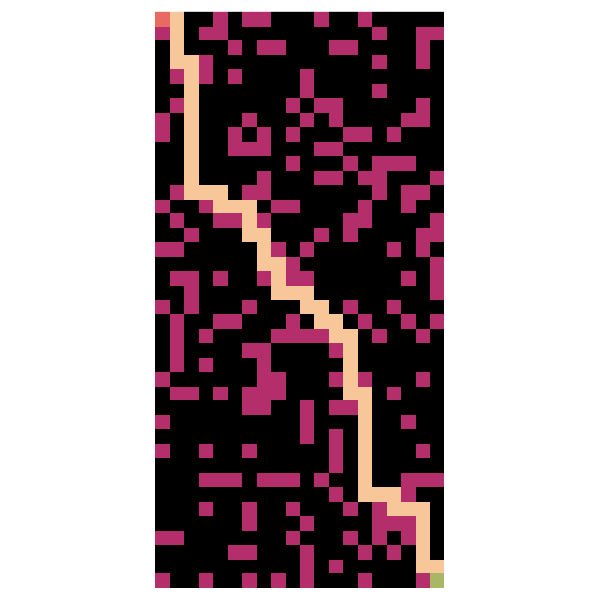
\includegraphics[scale=0.3]{../figures/path_03.png}
                \caption{4 vecinos (diagonales no permitidas); $\text{distancia} = 58 u$.}
            \end{subfigure}
            \hspace{1cm}
            %
            \begin{subfigure}{0.4\textwidth}
                \centering
                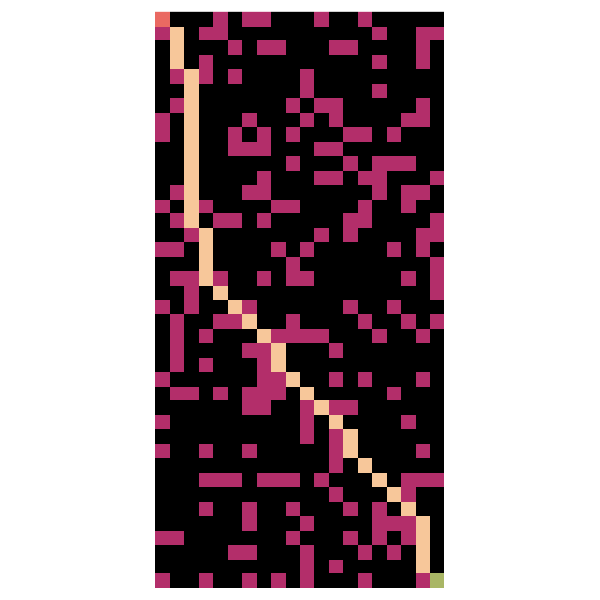
\includegraphics[scale=0.3]{../figures/path_03_diag.png}
                \caption{8 vecinos (diagonales no permitidas); $\text{distancia} = 46.87 u$.}
            \end{subfigure}
            \caption{Rejilla de $40 \times 20$ con una densidad de obstáculos del $25\%$.}
            \label{fig:rejilla_40x20}
        \end{figure}

        Para finalizar quisiera mostrar un caso en el que los obstáculos no se generan de manera aleatoria. No es el propósito explicar a detalle los pasos a continuación pero se hará lo mejor posible para que el lector pueda seguir los pasos. Primero, definimos el número de columnas y de filas que vamos a considerar para la imágen, también declaramos manualmente un color guardado en la variable \code{color\_} para identificar a los obstáculos\footnote{Corresponde al mismo color mostrado en las imágenes anteriores.} y se debe crear el vecindario, esto es, la imágen que contiene a todos los pixeles inicializados en negro \code{nh}:
        \begin{minted}[
            frame=none,
            autogobble,
            obeytabs=false,
            breaklines,
            tabsize=4,
            linenos=true,
            baselinestretch=1,
            firstnumber=1,
            bgcolor=bg!70,
            ]{julia}
            julia> color_ = sp.RGB(0.70196, 0.18039, 0.41568);
            julia> nh = zeros(sp.RGB, nrows, ncols);
        \end{minted}

        \begin{figure}[ht!]
            \centering
            \begin{subfigure}{0.4\textwidth}
                \centering
                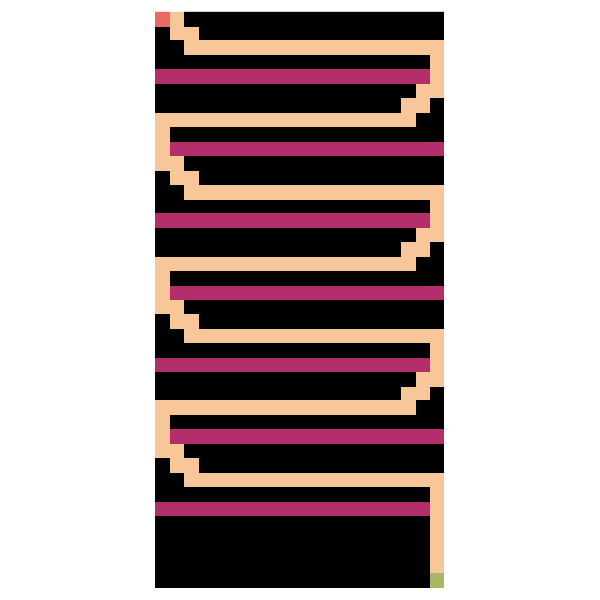
\includegraphics[scale=0.3]{../figures/escalera_nodiag.png}
                \caption{4 vecinos (diagonales no permitidas); $\text{distancia} = 172 u$.}
            \end{subfigure}
            \hspace{1cm}
            %
            \begin{subfigure}{0.4\textwidth}
                \centering
                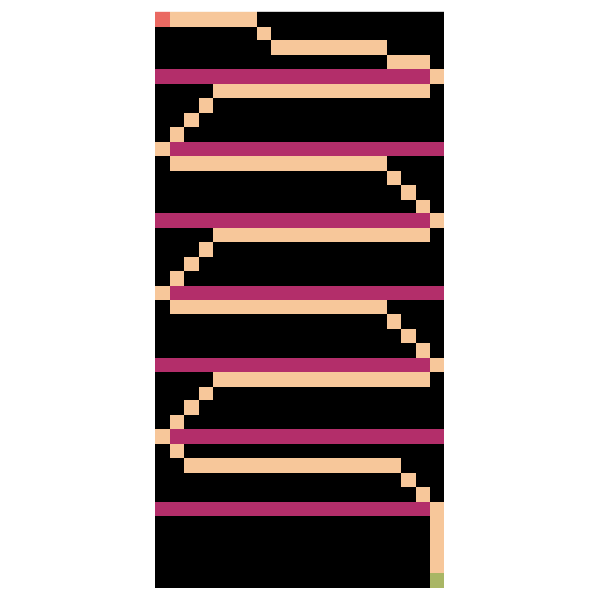
\includegraphics[scale=0.3]{../figures/escalera_diag.png}
                \caption{8 vecinos (diagonales no permitidas); $\text{distancia} = 152.08 u$.}
            \end{subfigure}
            \caption{Rejilla de $40 \times 20$ con una densidad de obstáculos del $16\%$.}
            \label{fig:rejilla_escalera}
        \end{figure}

        Se está considerando un arreglo similar al mostrado en la \cref{fig:rejilla_40x20} con 40 filas y 20 columnas. Se crearan obstáculos en forma de escalera, el color de estos pixeles se cambiará al color que corresponde a los obstáculos:
        \begin{minted}[
            frame=none,
            autogobble,
            obeytabs=false,
            breaklines,
            tabsize=4,
            linenos=true,
            baselinestretch=1,
            firstnumber=last,
            bgcolor=bg!70,
            ]{julia}
            julia> nh[5,begin:end-1] .= color_;
            julia> nh[10,begin+1:end] .= color_;
            julia> nh[15,begin:end-1] .= color_;
            julia> nh[20,begin+1:end] .= color_;
            julia> nh[25,begin:end-1] .= color_;
            julia> nh[30,begin+1:end] .= color_;
            julia> nh[35,begin:end-1] .= color_;
        \end{minted}
        Los obstaculos se encuentran preguntando cuáles no son de color negro, esto se hace con \code{findall}, este comando da una lista de índices cumpliendo cierta condición. Para este caso, la condición es aquellos pixeles que no son negros:
        \begin{minted}[
            frame=none,
            autogobble,
            obeytabs=false,
            breaklines,
            tabsize=4,
            linenos=true,
            baselinestretch=1,
            firstnumber=last,
            bgcolor=bg!70,
            ]{julia}
            julia> obs = findall(x -> x != sp.RGB(0,0,0), nh) .|> x -> sp.id(x[1], x[2], ncols);
        \end{minted}

        Nótese que se convirtieron los índices que se obtendrían con \code{findall} a la representación de los índices de la que se habló anteriormente ya que la función \code{adhacencyMatrix} requiere que los obstáculos se pasen como argumento en esta representación. Habiéndo dicho esto, se procede a calcular la matriz de adyacencia para ambos casos, cuando se permite moverse en diagonales y cuando no:
        \begin{minted}[
            frame=none,
            autogobble,
            obeytabs=false,
            breaklines,
            tabsize=4,
            linenos=true,
            baselinestretch=1,
            firstnumber=last,
            bgcolor=bg!70,
            ]{julia}
            julia> adjmat = sp.adjacencyMatrix(nrows, ncols; obstacles=obs, allowdiags=false);
            julia> adjmatdiag = sp.adjacencyMatrix(nrows, ncols; obstacles=obs, allowdiags=true);
            julia> path, dist = sp.findPath(adjmat, ncols; start=start, finish=finish);
            julia> pathdiag, distdiag = sp.findPath(adjmatdiag, ncols; start=start, finish=finish);
        \end{minted}

        Finalmente, se actualiza los vecindarios originales para incluir los caminos, y se guardan las imágenes:
        \begin{minted}[
            frame=none,
            autogobble,
            obeytabs=false,
            breaklines,
            tabsize=4,
            linenos=true,
            baselinestretch=1,
            firstnumber=last,
            bgcolor=bg!70,
            ]{julia}
            julia> sp.updateneighborhood!(nh, path)
            julia> sp.updateneighborhood!(nhdiag, pathdiag)
            julia> sp.savefig(fig, "../figures/escalera_nodiag.png");
            julia> sp.savefig(figdiag, "../figures/escalera_diag.png");
        \end{minted}

        En la \cref{fig:rejilla_escalera} se muestran ambos casos, cuando no se está permitido moverse en diagonales y cuando sí lo está permitido. A pesar de que no esté implementado en el módulo escrito elegir pixeles de manera interactiva, se pueden definir obstáculos de esta manera para generar estructuras más interesantes para las cuales encontrar sus caminos más cortos. Se invita al lector, estudiante o no, que juegue con esta funcionalidad para generar alún tipo de laberinto sencillo.
    \end{solution}
\end{enumerate}

\clearpage
\section*{Apéndice}
\inputminted[
    frame=none,
    autogobble,
    obeytabs=false,
    breaklines,
    tabsize=4,
    linenos=true,
    % numbersep=-10pt,
    baselinestretch=1,
    firstnumber=1,
    bgcolor=bg!70,]{julia}{\codepath}

\nocite{*} % to call all references even if they are not cited in the text
\bibliography{references.bib}

\end{document}